\section{Решение начально-краевой задачи для дифференциальных уравнений в частных производных параболического типа}

\subsection{Постановка задачи}
Используя явную и неявную конечно-разностные схемы, а также схему Кранка-Николсона, решить начально-краевую задачу для дифференциального уравнения параболического типа. Осуществить реализацию трех вариантов аппроксимации граничных условий, содержащих производные: двухточечная аппроксимация с первым порядком, трехточечная аппроксимация со вторым порядком, двухточечная аппроксимация со вторым порядком. В различные моменты времени вычислить погрешность численного решения путем сравнения результатов с приведенным в задании аналитическим решением $U(x, t)$. Исследовать зависимость погрешности от сеточных параметров $\tau$, $h$.

{\bfseries Вариант:} 10
\begin{align*}
& \frac{\partial u}{\partial t} = a \frac{\partial^2 u}{\partial x^2} + b \frac{\partial u}{\partial x} + c u,\ a > 0,\ b > 0,\ c < 0 \\
& u_x(0, t) + u(0, t) = \exp((c - a) t)(\cos(bt) + \sin(bt)) \\
& u_x(\pi, t) + u(\pi, t) = -\exp((c - a) t)(\cos(bt) + \sin(bt)) \\
& u(x, 0) = \sin x \\
& U(x, t) = \exp((c - a) t) \sin(x + bt) \\
\end{align*}
\pagebreak

\subsection{Результаты работы}
\begin{figure}[h!]
\centering
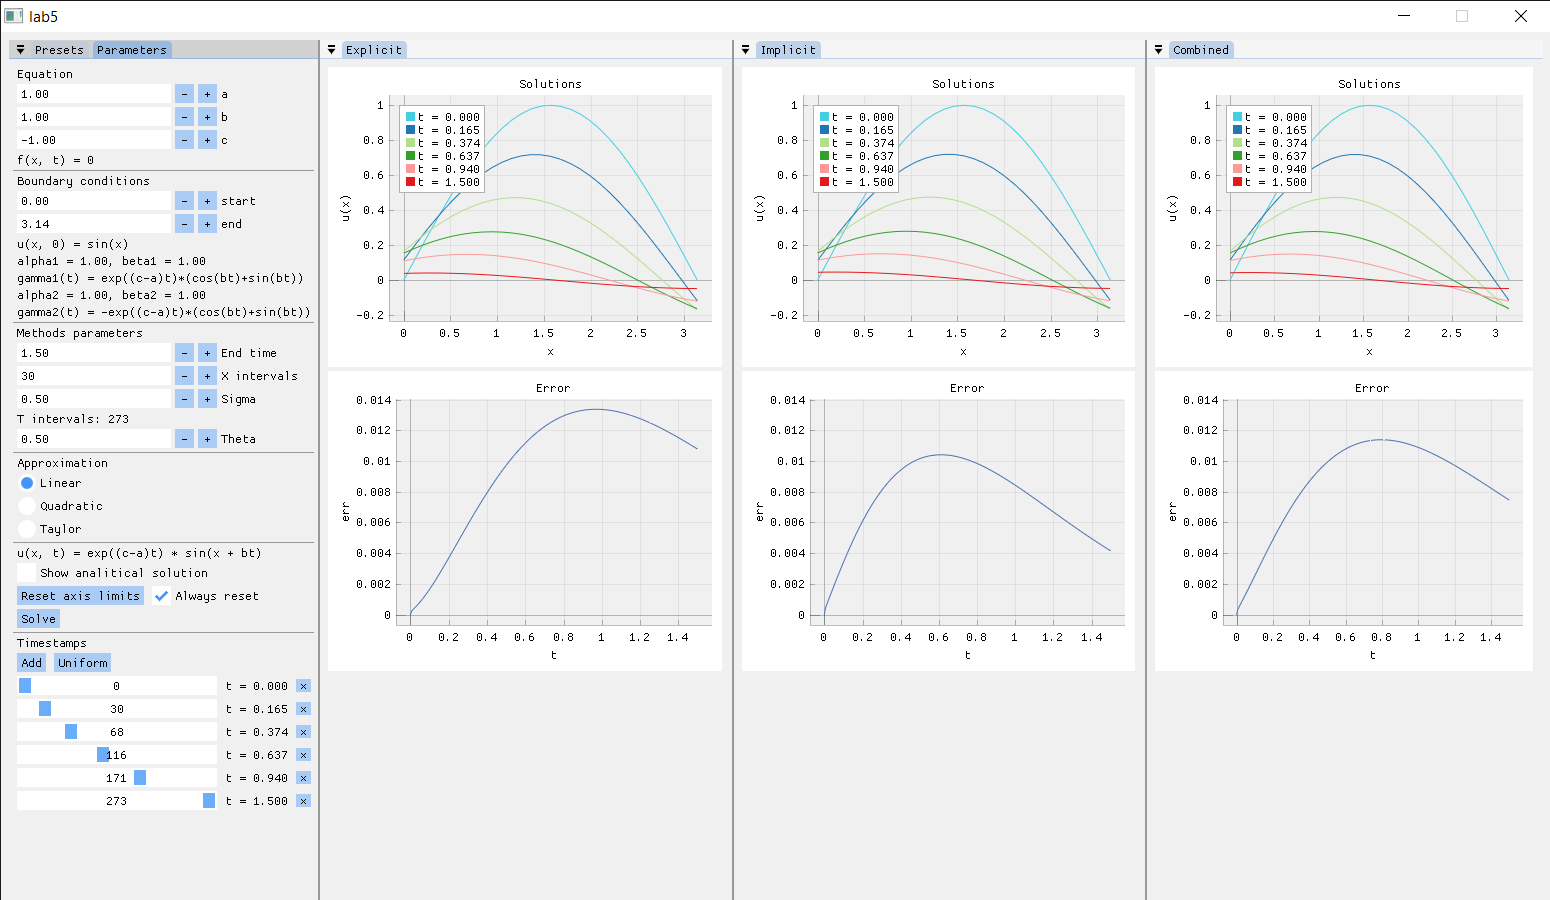
\includegraphics[width=.9\textwidth]{lab5_linear}
\caption{Решение с аппроксимацией граничных условий с первым порядком}
\end{figure}

\vfill

\begin{figure}[h!]
\centering
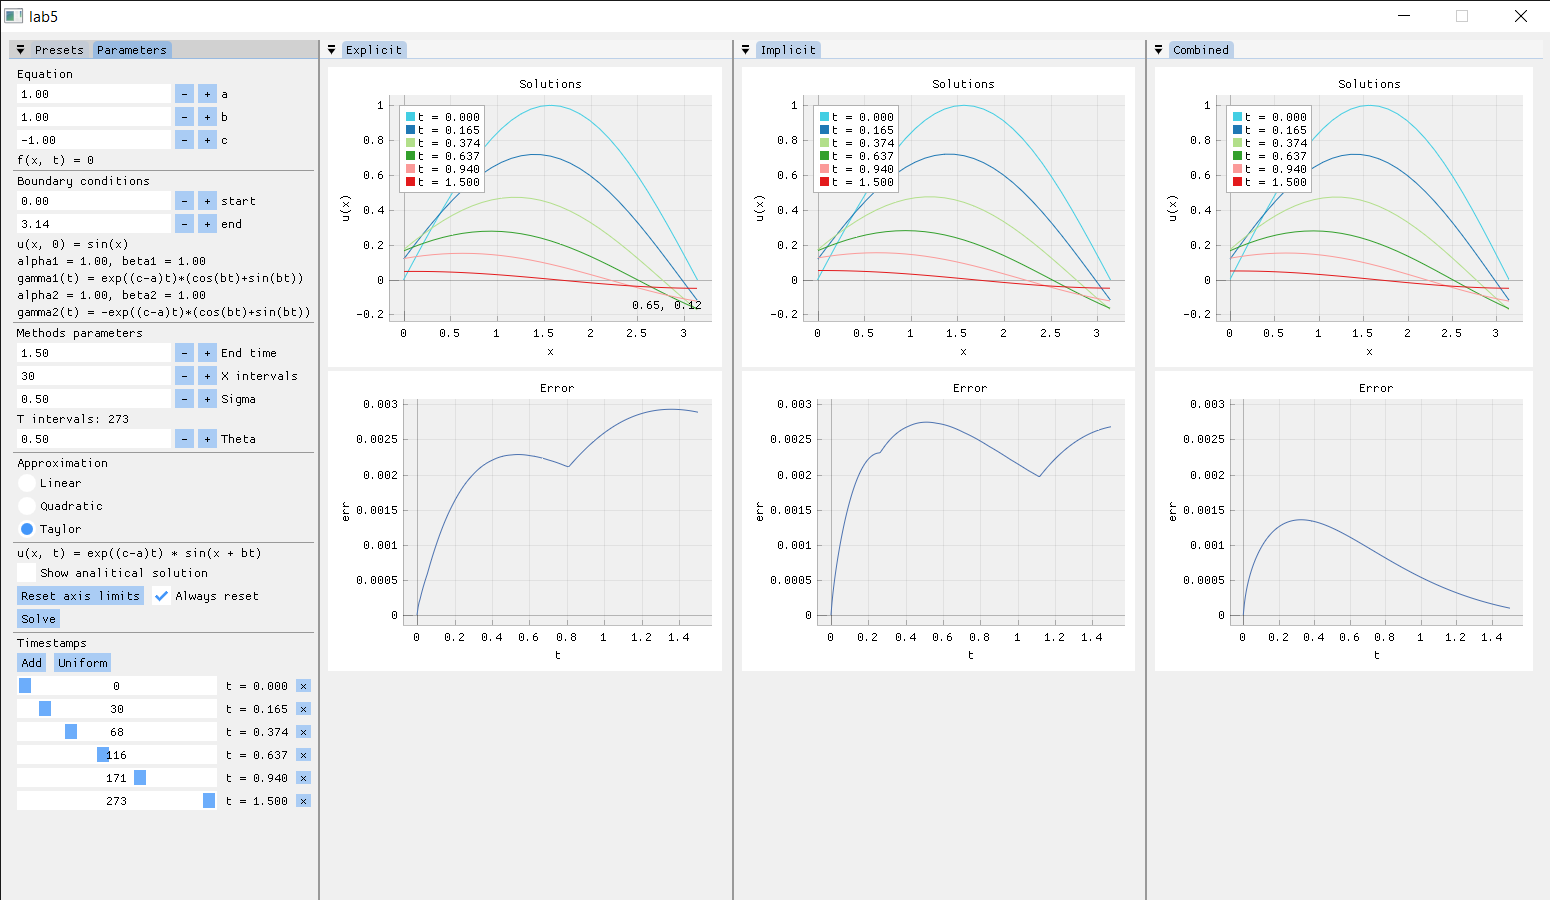
\includegraphics[width=.9\textwidth]{lab5_taylor}
\caption{Решение с аппроксимацией граничных условий со вторым порядком}
\end{figure}
\pagebreak

\subsection{Исходный код}
\lstinputlisting[title=\texttt{common.hpp}]{../../include/partial_differential/common.hpp}
\pagebreak
\lstinputlisting[title=\texttt{parabolic\_pde.hpp}]{../../include/partial_differential/parabolic_pde.hpp}
\pagebreak
